\documentclass[a4paper]{article}
\usepackage[]{enumerate} 
\usepackage[]{graphicx} 
\usepackage[]{subcaption} 
\usepackage[]{amsthm, amsmath, amssymb} 
\usepackage[]{fancyhdr}
\usepackage[]{hyperref} 
\urlstyle{sf}
\graphicspath{{../pictures/}}

\renewcommand{\vec}[1]{\mathbf{#1}}

\title{%
    \textsc{Atomic modeling of argon}\\
    \footnotesize{\textsc{Project 5 --- FYS3150}}
}
\author{%
    Ivar Haugal{\o}kken Stangeby\\
    \footnotesize{\textsc{Candidate no. 30}}
}

\begin{document}
\maketitle    

\begin{figure}[h]
    \centering
    
\includegraphics[width=\linewidth]{ch.pdf}
\end{figure}

\begin{abstract}
    In this project we explore the world of molecular dynamics. We are first
    presented with the skeleton of a working MD-program, and we are asked to
    implement the functionality we need as we go along. We look at the time
    evolution of a system of argon, with an initial face-centered cubic lattice
    configuration. The atoms are under the influence of the Lennard-Jones
    potential. We use the Velocity-Verlet as our time integrator of choice, and
    we compare this to the Euler-Cromer method in terms of energy conservation
    properties. We also compute the melting temperature of argon, by means of
    the Einstein relation and diffusion constant.
\end{abstract}
\tableofcontents
\listoffigures      

\section{Introduction}
\label{sec:introduction}
    Molecular dynamics (referred to as MD), deals with the time evolution of a
    system of particles, typically atoms or molecules. Being first explored in
    the late 1950's, it has had a wide range of applications, in fields as
    materials science, biochemistry and biophysics. It is based on the simple
    idea of considering a finite number of molecules and letting them interact
    for a fixed amount of time, which gives us an idea of how the system
    evolves. 

    In this project we examine what goes into creating a working MD-program
    that can compute various physical quantities and then proceed by
    considering some specific systems where we look at, amongst other, the
    kinetic energy, the initial temperature required in order to reach a
    desired final temperature, and finding the diffusion constant for the
    system in order to compute the melting temperature.

    The construction of the program will be covered in section
    \ref{sec:building_a_working_md_program}, where some of the motivation
    behind each addition to the program will be discussed. In section
    \ref{sec:simulations} we employ our newly implemented program and look at
    some specific systems.

\section{Building a working MD-program}
\label{sec:building_a_working_md_program}
    
    Initially, we are presented with the skeleton of a MD-program, and we are
    tasked with filling in the blanks. In this section, we walk through each of
    the steps that went into the implementation of the program, from skeleton
    to working program. The process can be summarized as following:
    
    \begin{enumerate}[1)]
        \item Introduce periodic boundary conditions.
        \item Implement a function for setting the net-momentum for the system to zero.
        \item Make the atoms conform to a face-centered cubic lattice configuration.
        \item Introduce the force model to the system, given by the Lennard-Jones potential.
        \item Implement the Velocity-Verlet algorithm in order to get a better
            conservation of energy.
        \item Write functions for sampling and storing physical quantities.
        \item Miscellaneous changes.
    \end{enumerate}
    
    Running the program in its initial state yields a random configuration of
    the atoms. Since there is no force acting on the molecules they move in
    straight lines determined by their initial velocity vector. Their motion is
    unbounded, due to the periodic boundary condition not being implemented
    yet. This can be seen in figure \ref{fig:first_iteration}.

    \begin{figure}
        \centering 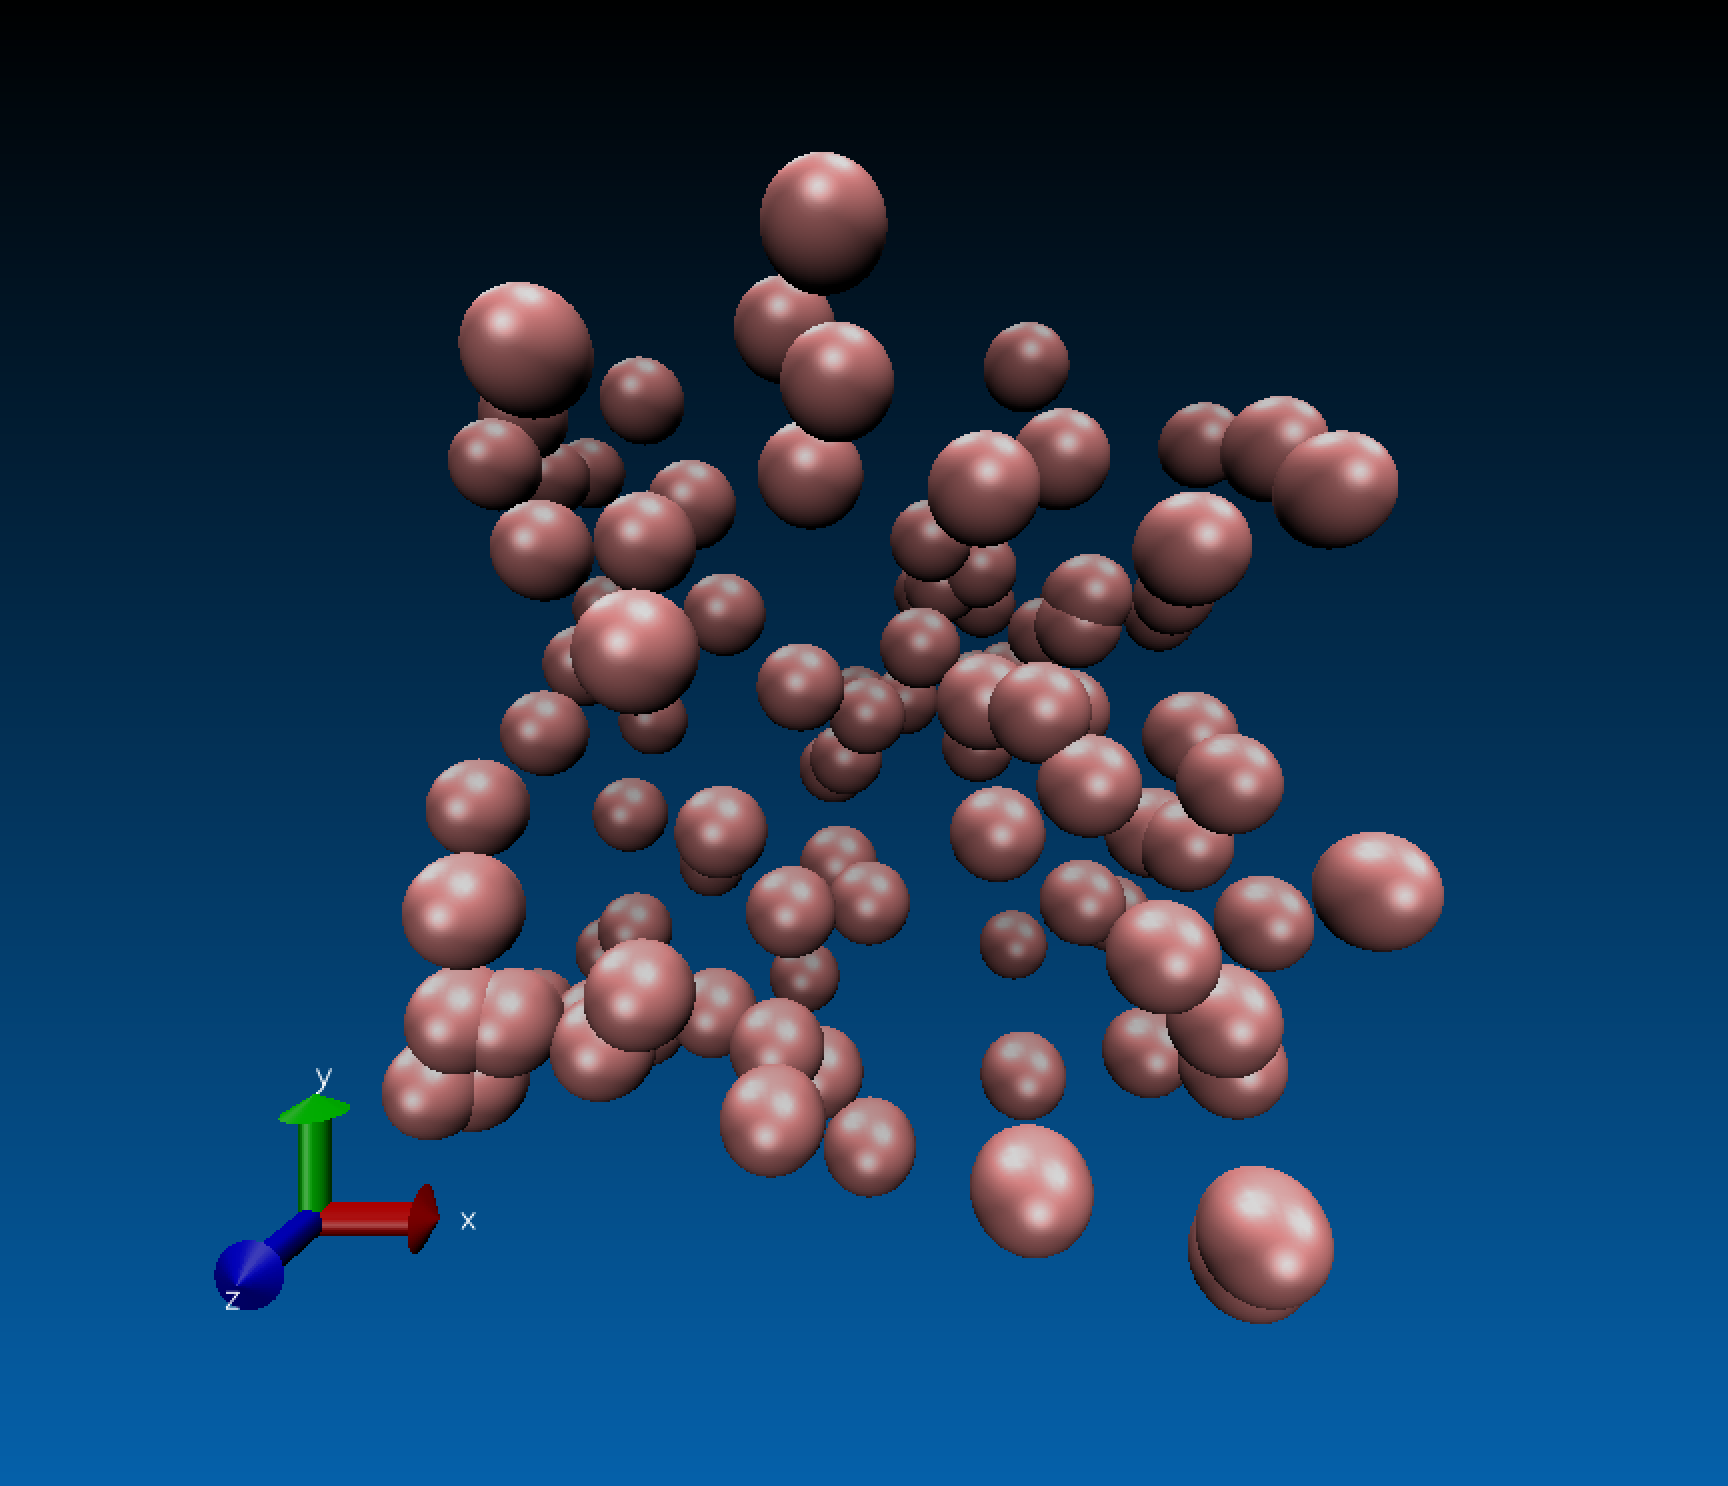
\includegraphics[width=0.4\linewidth]{first_iteration.png}
        \caption[Initial state of the program]{First iteration of the program --- no boundary conditions and
            no force acting on the atoms. The atoms move with a constant speed
            in the direction of their initial velocity and the initial
        positions are uniformly distributed.}
        \label{fig:first_iteration}
    \end{figure}

\subsection{Periodic boundary conditions}
\label{sub:periodic_boundary_conditions}
        
    We want our system to conform to periodic boundary conditions. The reasons
    for doing this is that a finite system with periodic boundary condition
    more closely resembles that of an infinite size. It is important that the
    bounding box which determines the boundary of the system is of sufficient
    size, so we do not get artifacts that arise from the fact that an atom can
    interact with itself. 
    
    There are two approaches to the implementation of periodic boundary
    condition. The most basic, and the one we will employ here is to have an
    atom exit through one face of the bounding box, and reappear through the
    opposite face. 

    Another approach is to not restrict the coordinates of the atom using the
    bounding box, and instead use the \emph{periodic image} of the atom when
    calculating interactions with ''nearby'' particles.
    
    We implement the function \texttt{applyPeriodicBoundaryConditions} in the
    \texttt{System}-class.  Our method is simply iterating over each atom, and
    in the cases where we find an atom outside the bounding box, we
    add/subtract the size of the box. If we let the vector $\vec{r}_i$, with
    components $r_q$ for $q = x, y, z$, denote the position of atom $i$ at any
    given time, we simply let the position be governed by the following
    relation:
    \begin{equation}
        \notag
        r_q = \begin{cases}
            r_q + L_q, & r_q < 0; \\
            r_q - L_q, & r_q > L_q; \\
            r_q, & \text{else.}
        \end{cases}
    \end{equation}
    Here $L_q$ is assumed to be the dimensions of the system in direction $q =
    x, y, z$.
    
    During simulations we need to be a bit cautious about what we define as the
    \emph{distance between} two atoms $i$ and $j$. Typically, we see this as
    the distance through the system, but due to our periodic boundary
    conditions there might be a shorter path through one of the borders of the
    system. This is formally stated as the \emph{minimum image
    criterion}\cite{min_image}.
    
\subsection{Zero out momentum}
\label{sub:zero_out_momentum}

    The Maxwell-Boltzmann distribution is good for velocities because it fairly
    accurately represents the way velocities are distributed in an ideal gas.
    The distribution was defined initially by Maxwell, for the specific purpose
    of describing particle speeds inside a stationary container with no
    interaction.  The distribution is directly dependent on the temperature of
    the system as well as the mass of each particle. We want to initialize each
    atom with a random velocity given by the Maxwell-Boltzmann distribution.

    Mathematically, the distribution function reads
    \begin{equation}
        \notag
        P(v_i)\, dv_i = \left( \frac{m_i}{2\pi k_BT} \right)^{1/2} e^{-\frac{mv_i^2}{2k_BT}}dv_i
    \end{equation}
    
    The problem that arises when using the Maxwell-Boltzmann distribution is
    that in its initial state the system has a non-zero net momentum. This
    causes the system to drift. This is why we want to implement the function
    \texttt{removeMomentum} in the \texttt{System}-class. Its purpose is to
    compute the total momentum of the system, and then remove a small portion
    of momentum from each atom in order to have a net momentum of zero. 
    
    We compute the velocity of the center of mass of the system, and then
    subtract this velocity from each atom.  Let $m_i$ and $v_i$ denote the mass
    and velocity of atom $i$ respectively and let $M$ and $V$ denote the total
    mass of the system and the velocity of the center of mass. Then
    \begin{align*}
        \notag
        V = \sum^{n}_{i=1} m_i v_i, \quad M = \sum^{n}_{i=1} m_i
    \end{align*}
    where $n$ is the total number of atoms in the system. We then need to
    subtract the value $V_{\mathrm{sub}} = V / M$ from each $v_i$.

\subsection{Face-centered cubic lattice}
\label{sub:face_centered_cubic_lattice}

    We now, instead of having random initial positions, want the atoms to form
    a crystal structure. In a face-centered cubic lattice (FCC), each unit cell
    has, in addition to the eight corner lattice points, one lattice point for
    each face.

    A \emph{unit cell} is a group of atoms which can be stacked on top and next
    to each other to form a grid structure. The \emph{lattice constant} defines
    the size of the unit cell, and is denoted $b$. In this project we are
    assuming cubic grids, so we let $N$ denote the number of unit cells in each
    dimension.
    
    We now define a local coordinate system for each unit cell as
    \begin{align*}
        \vec{r}_1 &= 0\hat{\vec{i}} + 0\hat{\vec{j}} + 0\hat{\vec{k}}, &
        \vec{r}_2 &= \frac{b}{2}\hat{\vec{i}} + \frac{b}{2}\hat{\vec{j}} +
        0\hat{\vec{k}},\\ \vec{r}_3 &= 0\hat{\vec{i}} +
        \frac{b}{2}\hat{\vec{j}} + \frac{b}{2}\hat{\vec{k}}, & \vec{r}_4 &=
        \frac{b}{2}\hat{\vec{i}} + 0\hat{\vec{j}} + \frac{b}{2}\hat{\vec{k}}.
    \end{align*}
    The origin for an arbitrary unit cell is then given (globally) as
    \begin{equation}
        \notag \vec{R}_{i, j, k} = i\hat{\vec{u}}_1 + j\hat{\vec{u}}_2 +
        k\hat{\vec{u}}_3
    \end{equation}
    We implement the function \texttt{createFFCLattice} in the
    \texttt{System}-class which takes $N$ and $b$ as arguments. The initial
    configuration for an example system is displayed in figure
    \ref{fig:ffc_iteration}.
    \begin{figure}
        \centering 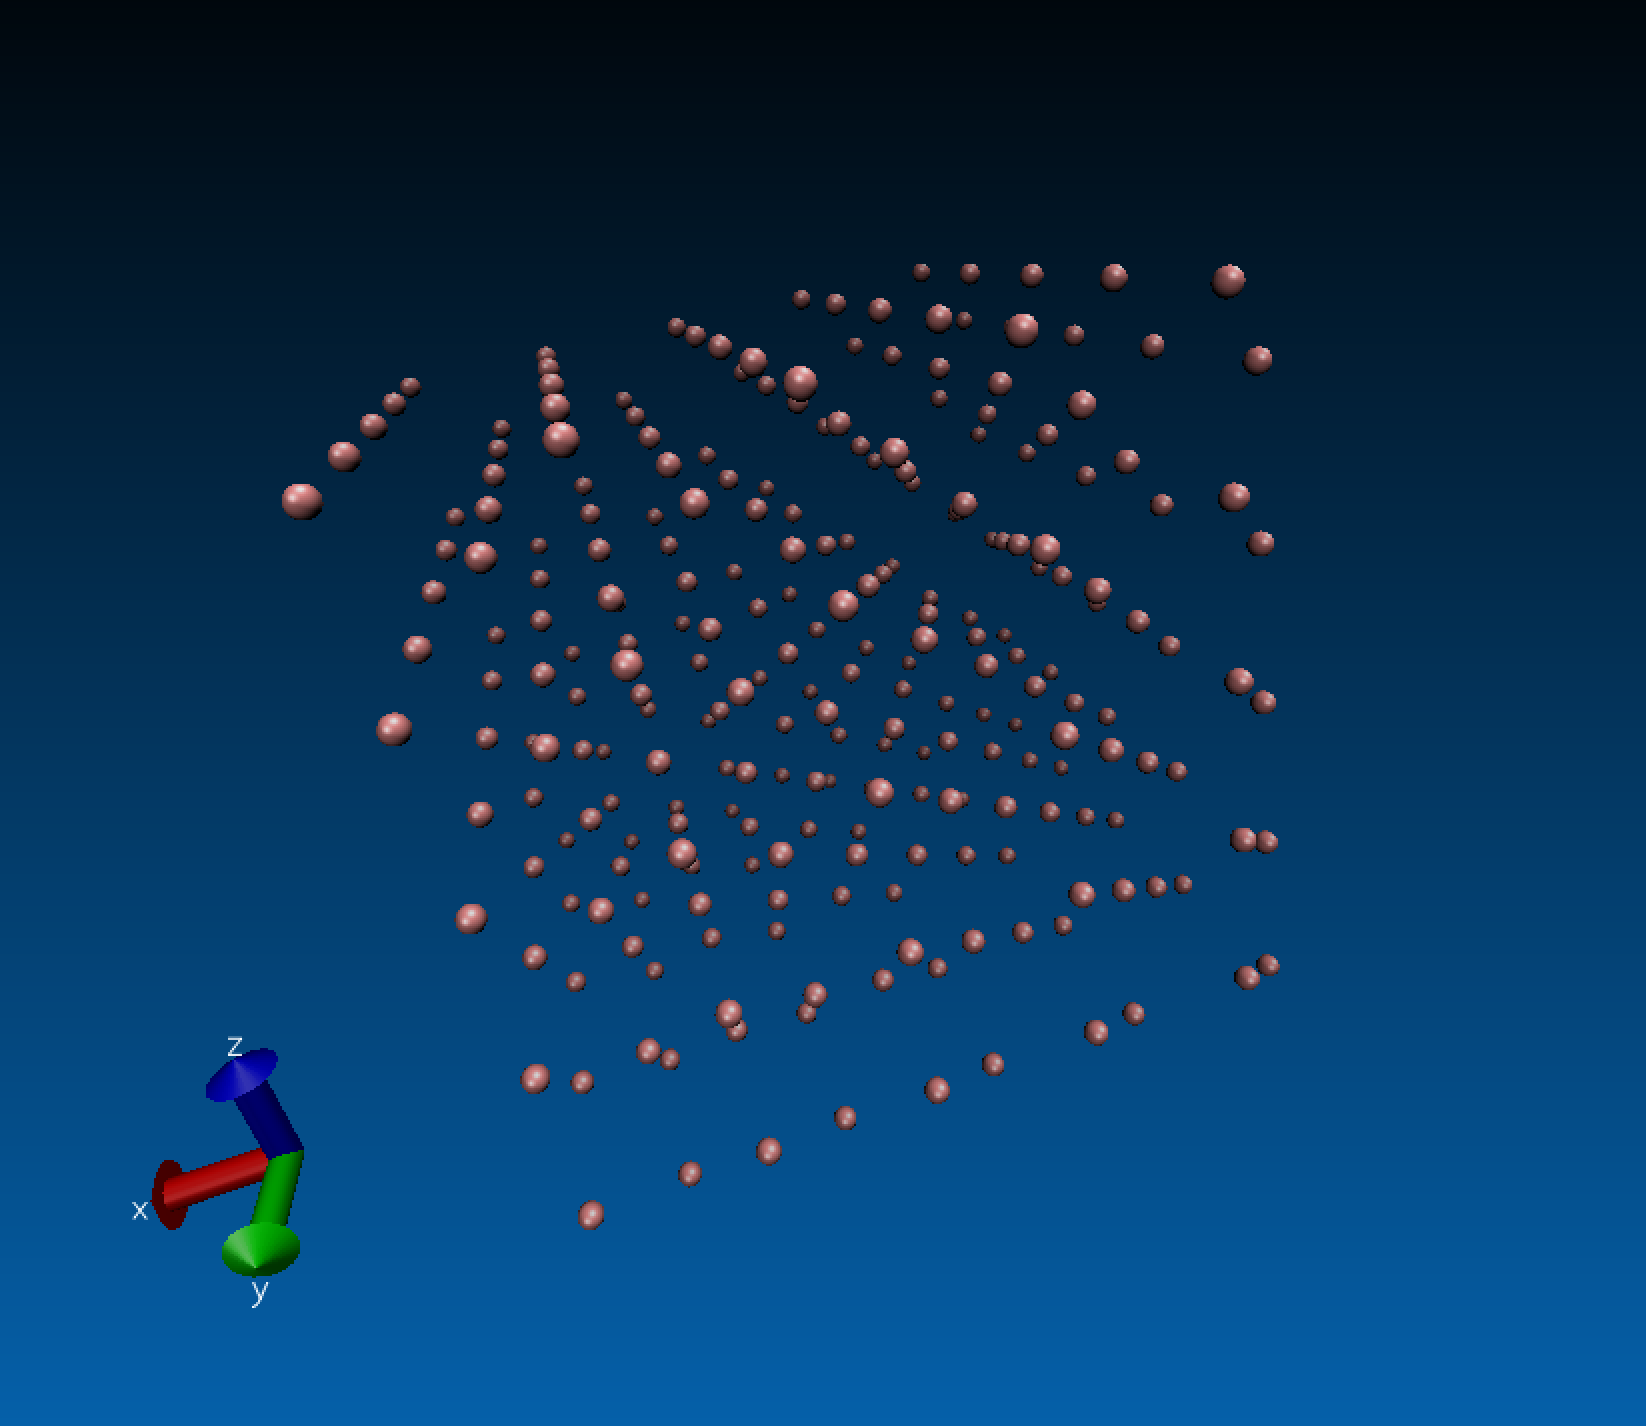
\includegraphics[width=0.4\linewidth]{ffc_iteration}
        \caption[Crystallic structure in argon]{Initial configuration of a
            FFC-based lattice. We have here used a lattice constant $b =
            5.26${\AA} and the number of unit cells in each dimension is $N =
            5$. This specific system has a density of $\rho = M / V = 4N^3m /
            b^3N^3$ where $m$ is the mass of each atom, $b$ and $N$ given as
            above. This evaluates to approximately $0.1445 \,\mathrm{a.m.u} /
        \mathrm{\AA}^3$.}
        \label{fig:ffc_iteration}
    \end{figure}
    
\subsection{Lennard-Jones potential}
\label{sub:lennard_jones_potential}

    The Lennard-Jones potential approximates the interaction between a pair of
    atoms. In its most common form it reads
    \begin{equation}
        \notag U(r_{ij}) = 4\varepsilon \left[ \left( \frac{\sigma}{r_{ij}}
        \right)^{12} - \left( \frac{\sigma}{r_{ij}} \right)^6 \right],
    \end{equation}
    where $r_{ij}$ is the distance between atom $i$ and atom $j$ and
    $\varepsilon$ is the depth of the potential well. The quantity $\sigma$ is
    the distance for which the potential is zero.  With an expression for the
    potential we can sum over all distinct pairs of atoms and acquire an
    expression for the total potential energy $V$:
    \begin{equation}
        \notag V = \sum^{}_{i>j}U(r_{ij}).
    \end{equation}
    The force exerted on atom $i$ by atom $j$ is then given as the negative
    gradient of the potential between the two:
    \begin{equation}
        \notag \vec{F}(r_{ij}) = -\nabla U(r_{ij}).
    \end{equation}
    The three force-components are given by:
    \begin{align*}
        F_q(r_{ij}) = -\frac{\partial U}{\partial r_{ij}} \frac{\partial
        r_ij}{\partial q_{ij}} \quad (q = x, y, z)
    \end{align*}
    Analytically, this evaluates to
    \begin{align*}
        F_q(r_{i, j}) = 24\varepsilon \left[ \left(
        \frac{2\sigma^{12}}{r_{ij}^{13}}\right) - \left(
        \frac{\sigma^6}{r_{ij}^7}\right)\right] \quad (q = x, y, z).
    \end{align*}
    The brute force way of computing this is summing over each distinct pair of
    atoms, and computing the mutual force between them. This however,
    constitutes a fairly heavy computational load that quickly scales with the
    size of the system. For a total of $n$ atoms in the system, we have a time
    complexity of $\mathcal{O}(n^2)$. Luckily more efficient methods are
    available, most notably is the Verlet list method. 
    
    We need to chose the parameters $\sigma$ and $\varepsilon$ so that they are
    suited for simulation of argon. It turns out that $\sigma = 3.405
    \mathrm{\AA}$ and $\varepsilon = 119.8k_B\mathrm{K}$ with $k_B = 1$ in
    MD-units.

    Argon has a melting point of $\approx 84$K and a boiling point of $\approx
    87$K. If we run the simulations, once for a temperature of $40$K, once for
    $85$K and finally once for $120K$ we should see indications of three
    different phases. The results shows that the model somewhat accurately
    manages to capture these phase transitions. Snapshots taken at the same
    point in time for all three cases are presented in figure
    \ref{fig:potential_iteration}.
    \begin{figure}
        \begin{tabular}[c]{ccc}
            \begin{subfigure}[c]{0.32\textwidth}
                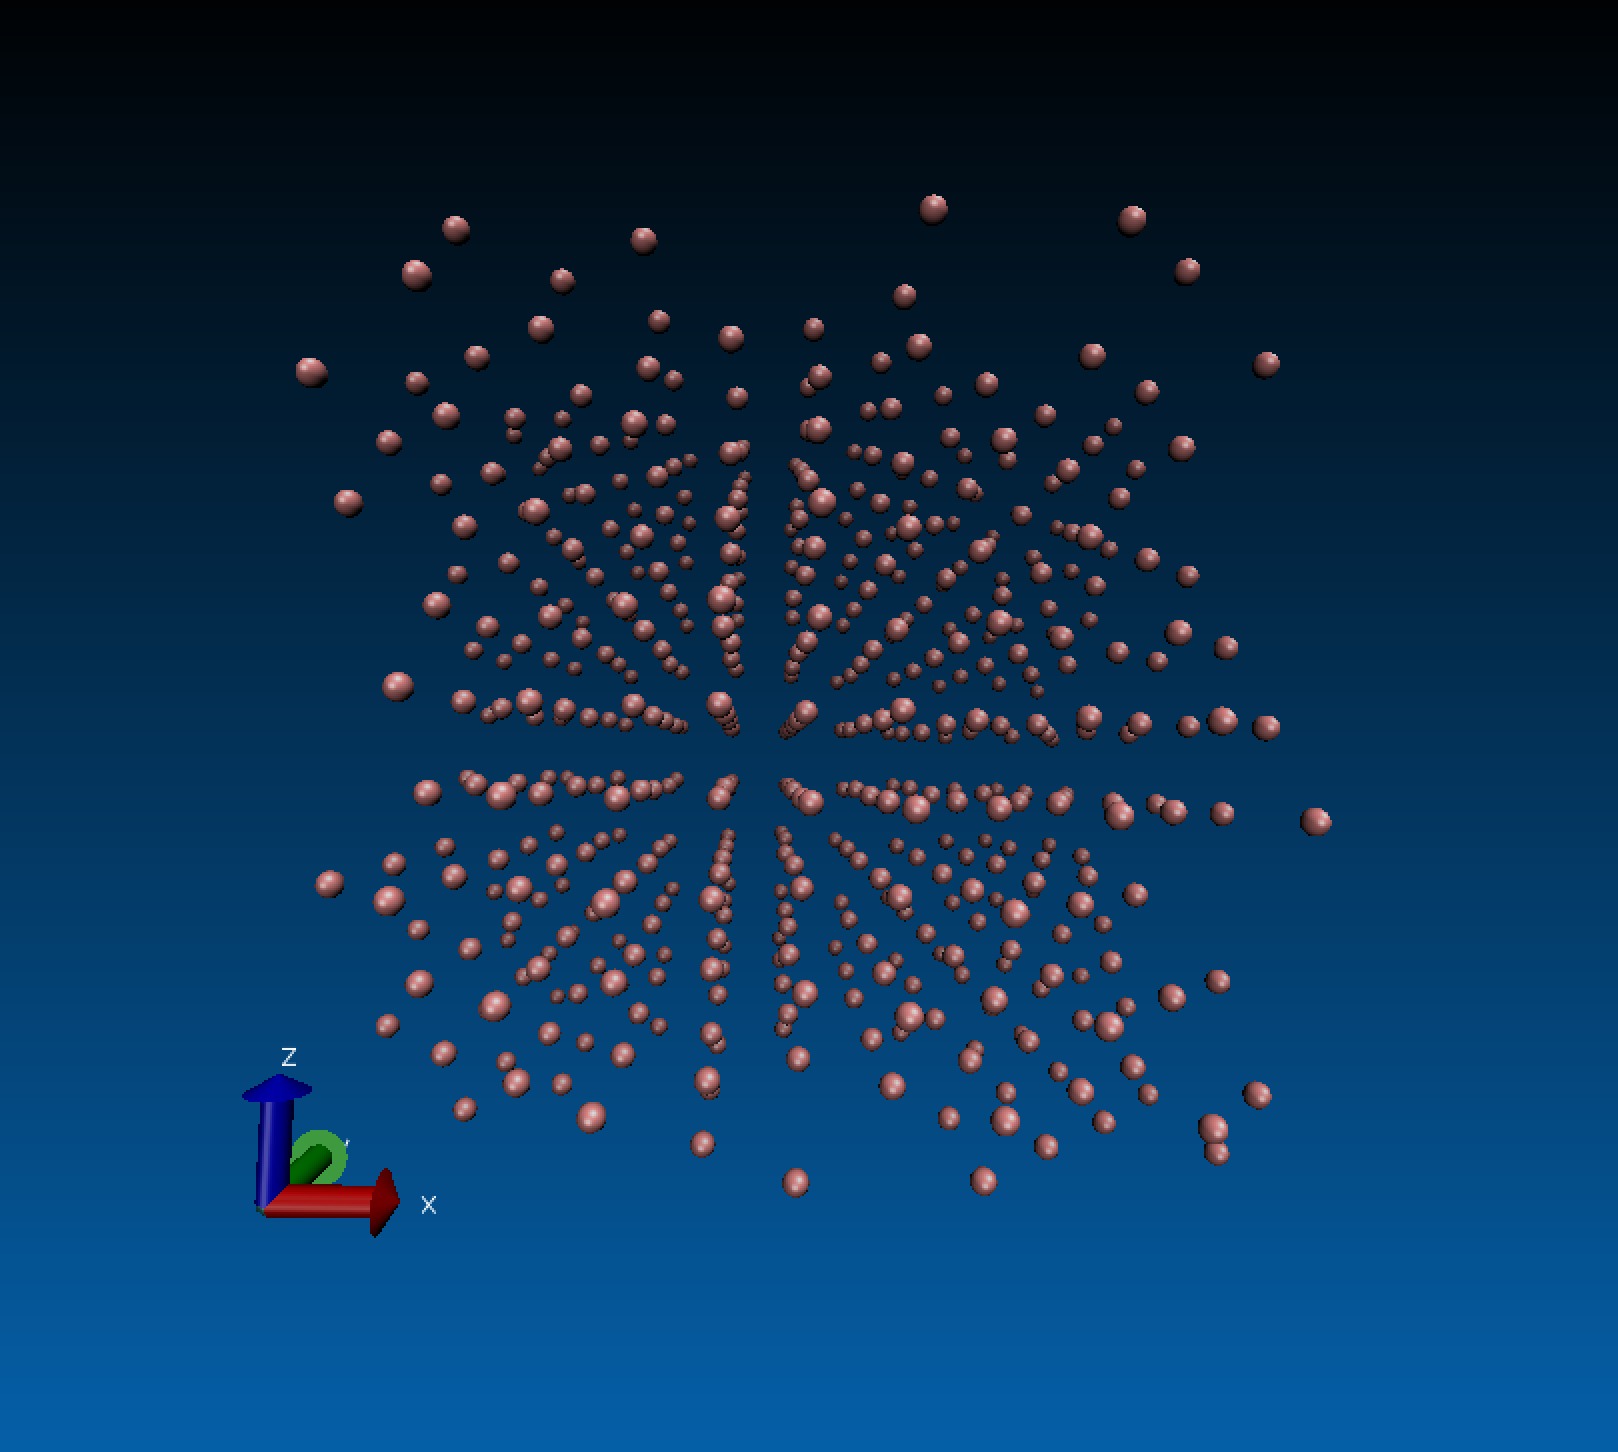
\includegraphics[height=100pt, width=\linewidth]{solid_40K.png}
                \caption{$T = 40$K}
            \end{subfigure}
            \begin{subfigure}[c]{0.32\textwidth}
                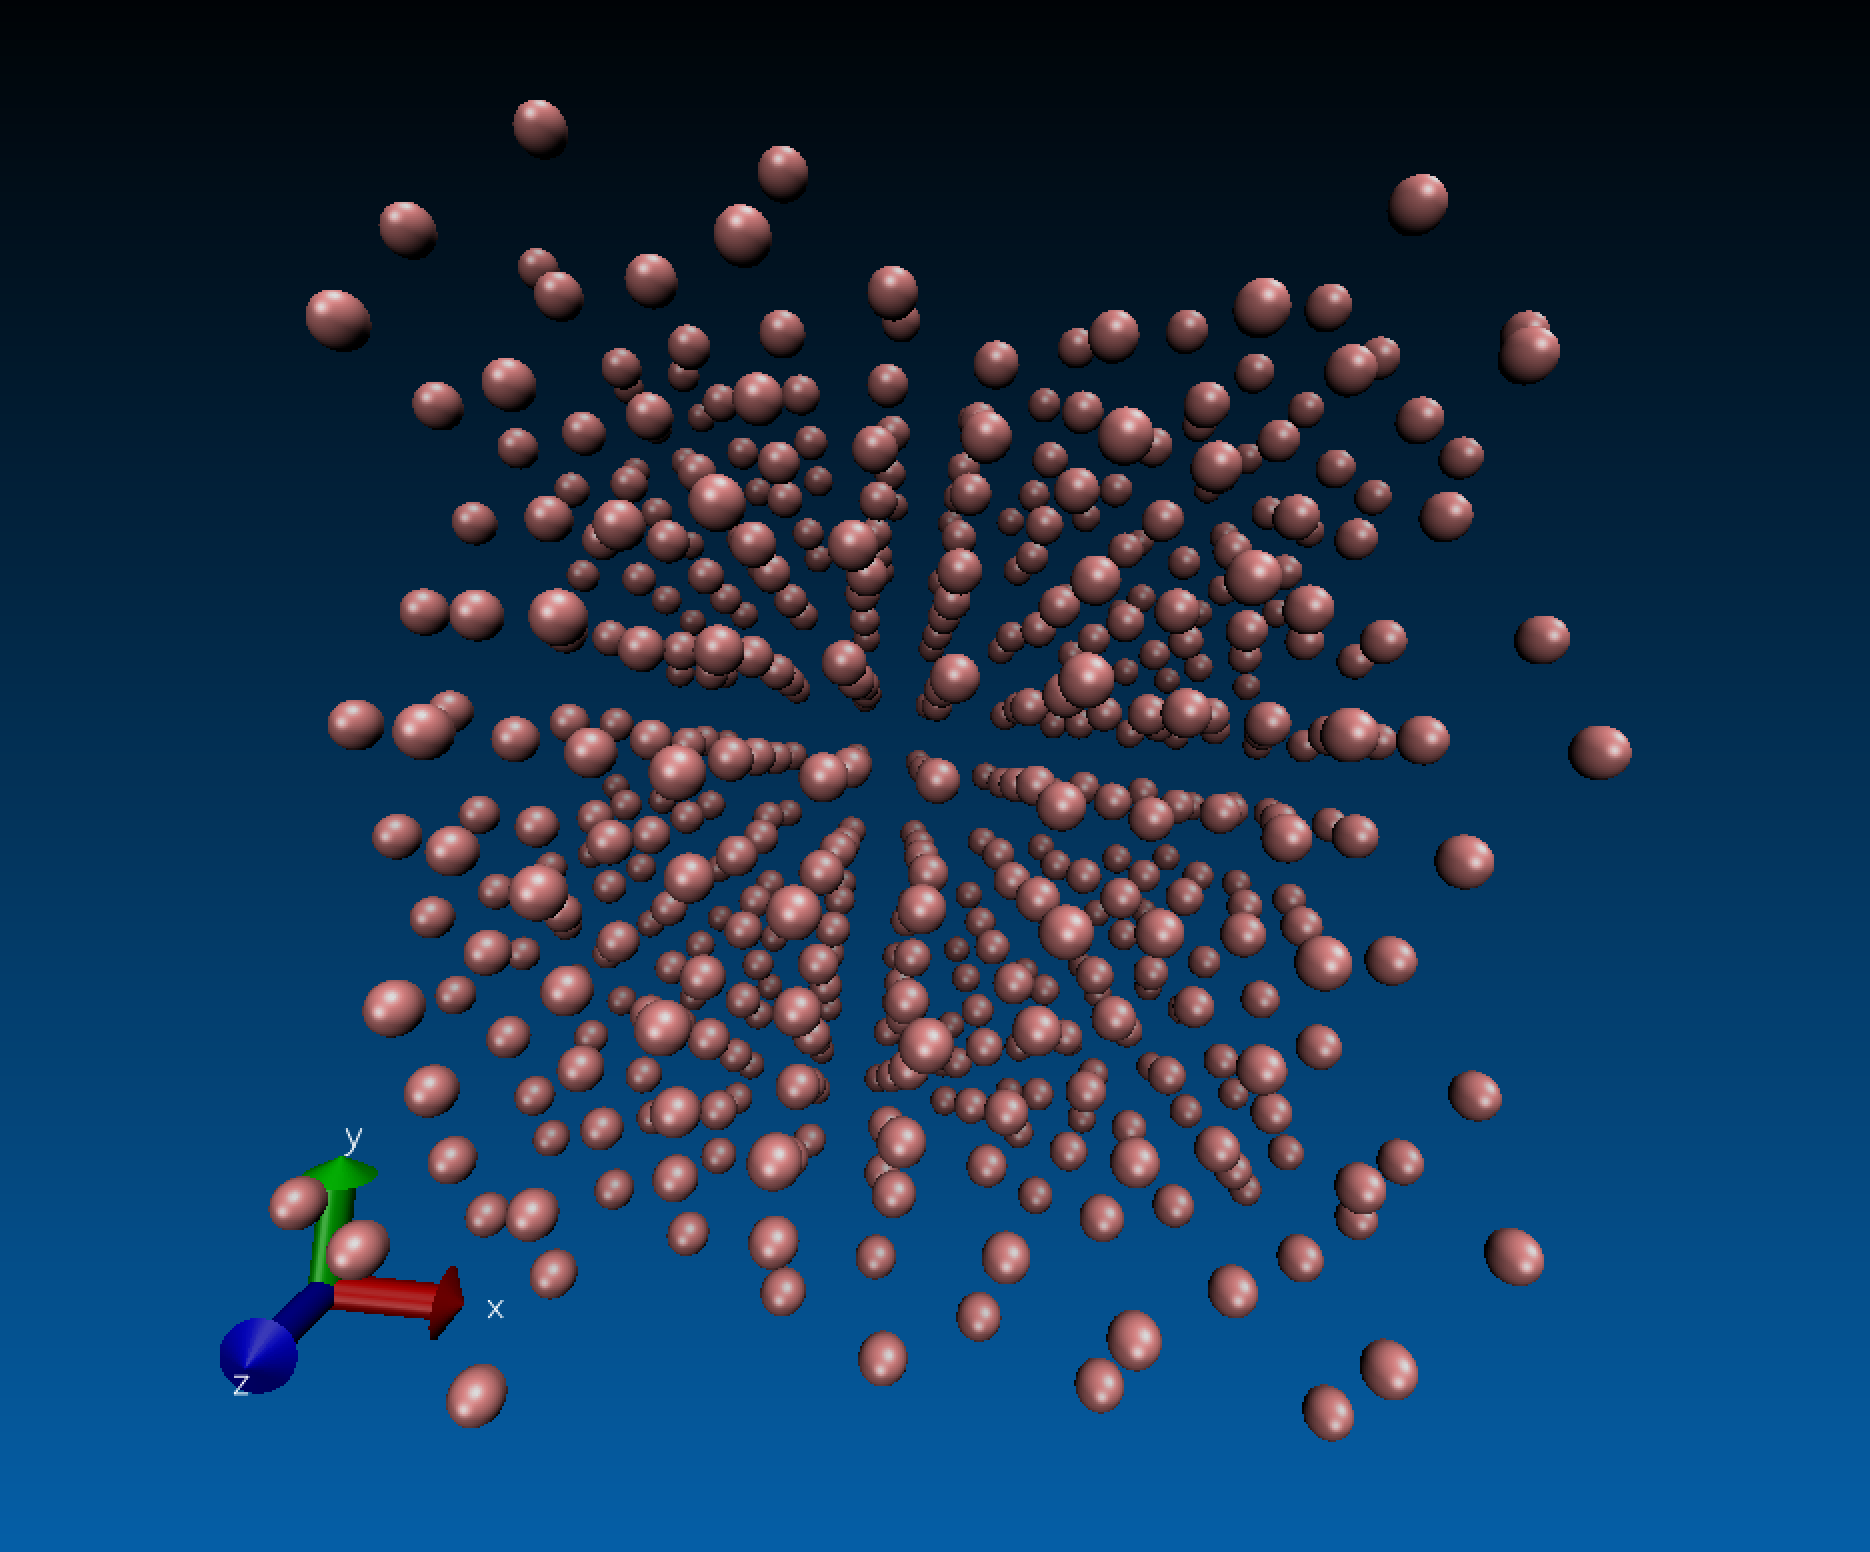
\includegraphics[height=100pt, width=\linewidth]{liquid_85K.png}
                \caption{$T = 85$K}
            \end{subfigure}
            \begin{subfigure}[c]{0.32\textwidth}
                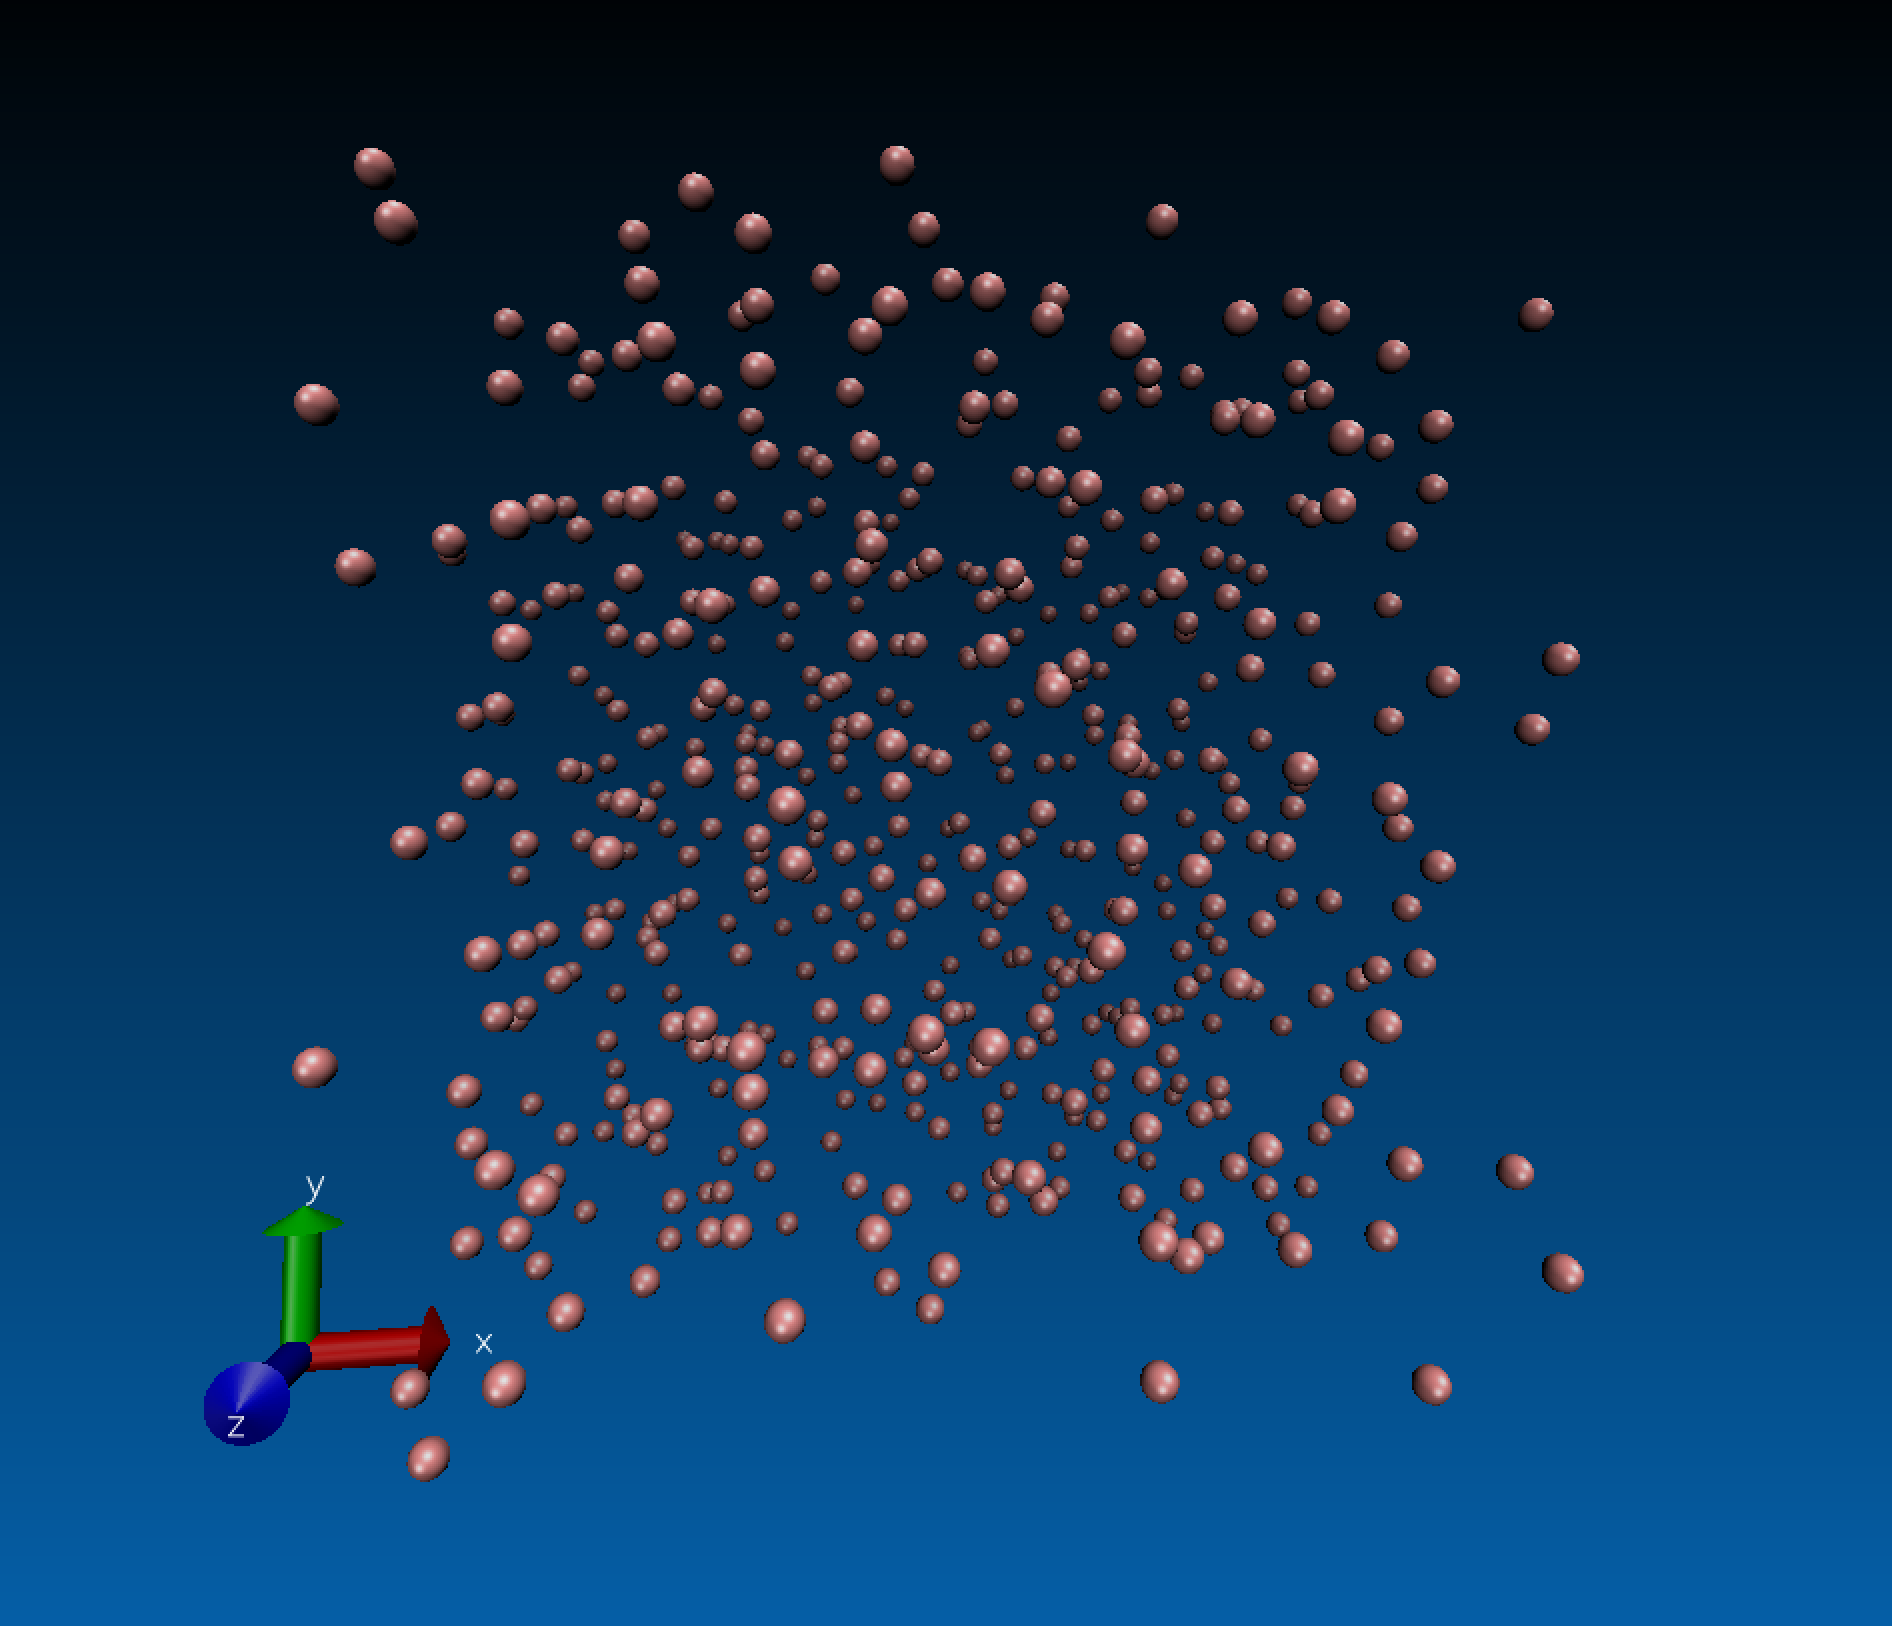
\includegraphics[height=100pt, width=\linewidth]{gas_120K.png}
                \caption{$T = 120$K}
            \end{subfigure}
        \end{tabular}
        \caption[Argon phases]{Snapshots taken of the system at frame 500/999 for
            temperatures of $40$, $85$ and $120$ kelvin. It is a bit difficult
            to conclude from the pictures, one really needs to see the system
            in motion, but the system do behave more or less like a solid, a
            liquid and a gas for respective temperatures. It is possible to see a
            certain change in the entropy of the system across the three
            images. These made use of the Velocity-Verlet integration method.}
        \label{fig:potential_iteration}
    \end{figure}

    \subsection{Velocity Verlet, a symplectic integrator}
    \label{sub:velocity_verlet_a_symplectic_integrator}
    
    In order to improve upon the fairly poor energy conservation of the
    Euler-Cromer method, we chose to implement the Velocity Verlet integrator.
    The algorithm is dependent on us having computed the forces for the first
    step and consists of three steps per time-step:
    \begin{align*}
        \vec{v}(t + \Delta t/2) &= \vec{v}(t) + \frac{\vec{F}(t)}{m}\frac{\Delta t}{2},\\
        \vec{r}(t + \Delta t) &= \vec{r}(t) + \vec{v}(t + \Delta t/2)\Delta t, \\
        \vec{v}(t + \Delta t) &= \vec{v}(t + \Delta t/2) + \frac{\vec{F}(t+\Delta t)}{m} \frac{\Delta t}{2}.
    \end{align*}
    We implement this algorithm in the \texttt{integrate} method in the
    \texttt{VelocityVerlet}-class. The method takes a system of atoms and a
    time step $\Delta t$ as arguments. We also introduce the private auxiliary
    variable \texttt{m\_first\_step}, which helps us take care of the initial
    calculation of the forces.
    
    Of interest now is how our new method of integration compares with the old
    one. One way of looking at this is by examining the fluctuations in the
    total energy as functions of the time step $\Delta t$. This will be
    examined in section \ref{sub:energy_conservation_of_integration_method}.
    
    \subsection{Sampling quantities}
    \label{sub:sampling_quantities}
   
    We now have pretty much a working program, however we still need to sample
    the physical properties of the system at each time step. For this we turn
    to the \texttt{StatisticsSampler}-class where we will implement the methods
    for sampling the density, kinetic and potential energy and temperature of
    the system. The methods are named accordingly.
    
    We first start by considering the kinetic and potential energy of the
    system. We already have computed the potential energy, in the
    \texttt{LennardJones}-class, so we are now interested in computing the
    kinetic energy. The kinetic energy of an arbitrary atom $i$ is defined as
    $E_{k}^i = m_iv_i^2/2$, and so the total kinetic energy $E_k$ of the system
    is simply
    \begin{equation}
        \notag
        E_k = \sum^{n}_{i=1} E_k^i = \sum^{n}_{i=1} \frac{1}{2}m_iv_i^2,
    \end{equation}
    where $m_i$ and $v_i$ is the mass and velocity atom $i$ and $n$ is again
    the total number of atoms in the system.
    
    We are also interested in the instantaneous temperature of the system, and
    the equipartition theorem \cite{equipar} can help us with this. The theorem
    relates the average energy of a system to its temperature and gives us the
    relation $\langle E_k \rangle = (3/2)k_BT$ which can be solved for
    temperature:
    \begin{equation}
        \notag
        T = \frac{2}{3} \frac{E_k}{nk_B}.
    \end{equation}
    Notice the removal of the brackets --- we are only interested in the
    \emph{instantaneous} temperature at any point in time. We also recall that
    since our units are scaled, Boltzmann's constant is equal to one.
    
    \subsection{Miscellaneous changes}
    \label{sub:miscellaneous_changes}
    
    In order to ease the implementation of the python framework used to run the
    simulations, we need to make some auxiliary changes to the
    \texttt{main}-method of the program. First of all, we are interested in
    comparing the two integration methods the program currently supports, so we
    add a fourth possible command line argument for setting the integration
    method. The program defaults to Velocity-Verlet.  
    
    We also need a way of changing the time step $\Delta t$ used in the
    simulations. This is also implemented as a command line argument, and we
    use a default time step of $\Delta t = 1.0 \times 10^{-15}$ seconds.
    
    In order to compute the \emph{mean square displacement} in section
    \ref{sub:melting_temperature_of_system} we need to keep track of the
    initial position of each atom. We therefore introduce a variable
    \texttt{m\_initialPosition} in the \texttt{Atom-class} which is set during
    initialization.  When computing the diffusion constant $D$, we need to make
    sure that $r_i^2(t)$ is the true displacement, and not the displacement
    relative to the nearest periodic image. This will be implemented in the
    \texttt{applyBoundaryConditions}-method.

\section{Simulations}
\label{sec:simulations}

In this section we consider various systems and simulate them using the program
devised in the previous section.

\subsection{Energy conservation of integration method}
\label{sub:energy_conservation_of_integration_method}

We initially decided to use the Velocity-Verlet integration method instead of
Euler-Cromer because of its good energy conservation. It is therefore of
interest to examine exactly what kind of impact this change of integration
method has for our simulations.  We now simulate a set of similar systems and
look at how the fluctuations in total energy scales with the time step $\Delta
T$. In order to do this we can consider the standard-deviation of the total
energy. 

We are going to run the simulations for a starting temperature of 300 kelvin,
and vary the time step from $1.0 \times 10^{-15}$ to $1.0 \times 10^{-14}$
seconds with 40 intermediate values. The results, as shown in figure
\ref{fig:energy_fluctuations}, tells us exactly how much better Velocity Verlet
is when it comes to energy conservation.

\begin{figure}[h]
    \centering 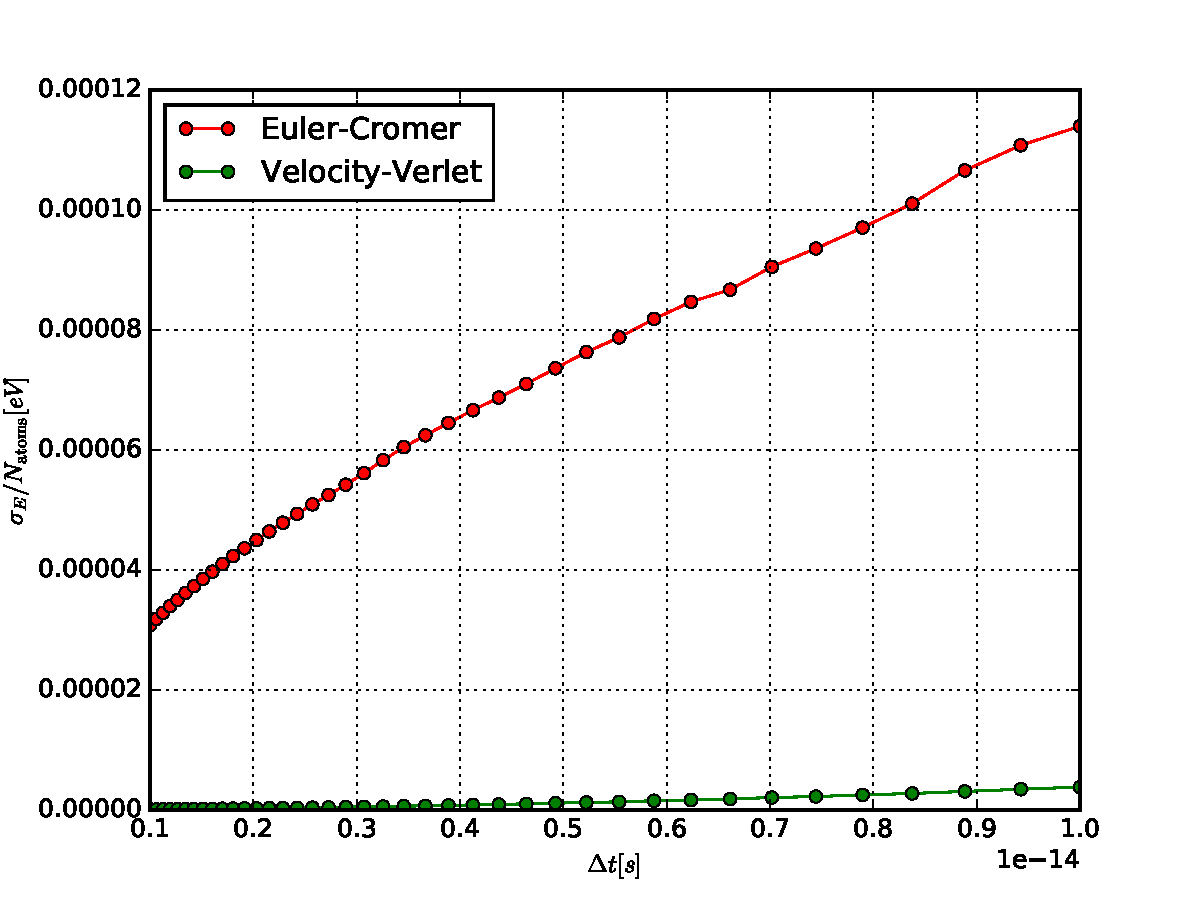
\includegraphics[width=0.8\linewidth]{energy_fluctuations.pdf}
    \caption[Energy fluctuations]{The standard deviation of the total energy as
        a function of the time-step $\Delta t$ with the energy being per atom.
        This clearly shows the benefits of using Velocity-Verlet over
    Euler-Cromer. While Euler-Cromer gives rise to fluctuations that scale
somewhat linearly in the time step $\Delta t$, the fluctuations attributed to
Velocity-Verlet is negligible in comparison.}
    \label{fig:energy_fluctuations}
\end{figure}

\subsection{Initial to final temperature}
\label{sub:initial_to_final_temperature}

We are now interested in determining what initial temperature $T_i$ is needed
in order to have a final temperature of $T$.  One way of examining this is by
looking at the ratio $T/T_i$. As we can see in figure \ref{fig:temperature_ratio} the
ratio stabilizes around $T/T_i = 0.5$. Solving this for $T_i$ tells us that if
we are interested in a final temperature of $T$, then we should chose our
initial temperature to be
\begin{equation}
    \notag
    T_i = 2T.
\end{equation}

As we see from the plot, the temperature drastically drops just after the
initial state. This is because $T \propto E_k$, i.e., the temperature is
proportional to the kinetic energy, and since the potential has not yet kicked
in, the kinetic energy is at its maximum. While what we have just observed is
an empirical result, we can alternatively look at the virial theorem
\cite{virial}, which relates the time average of the kinetic energy to the time
average of the potential energy. This gives us a description of this
stabilization independent of the temperature. 

\begin{figure}[h]
    \centering 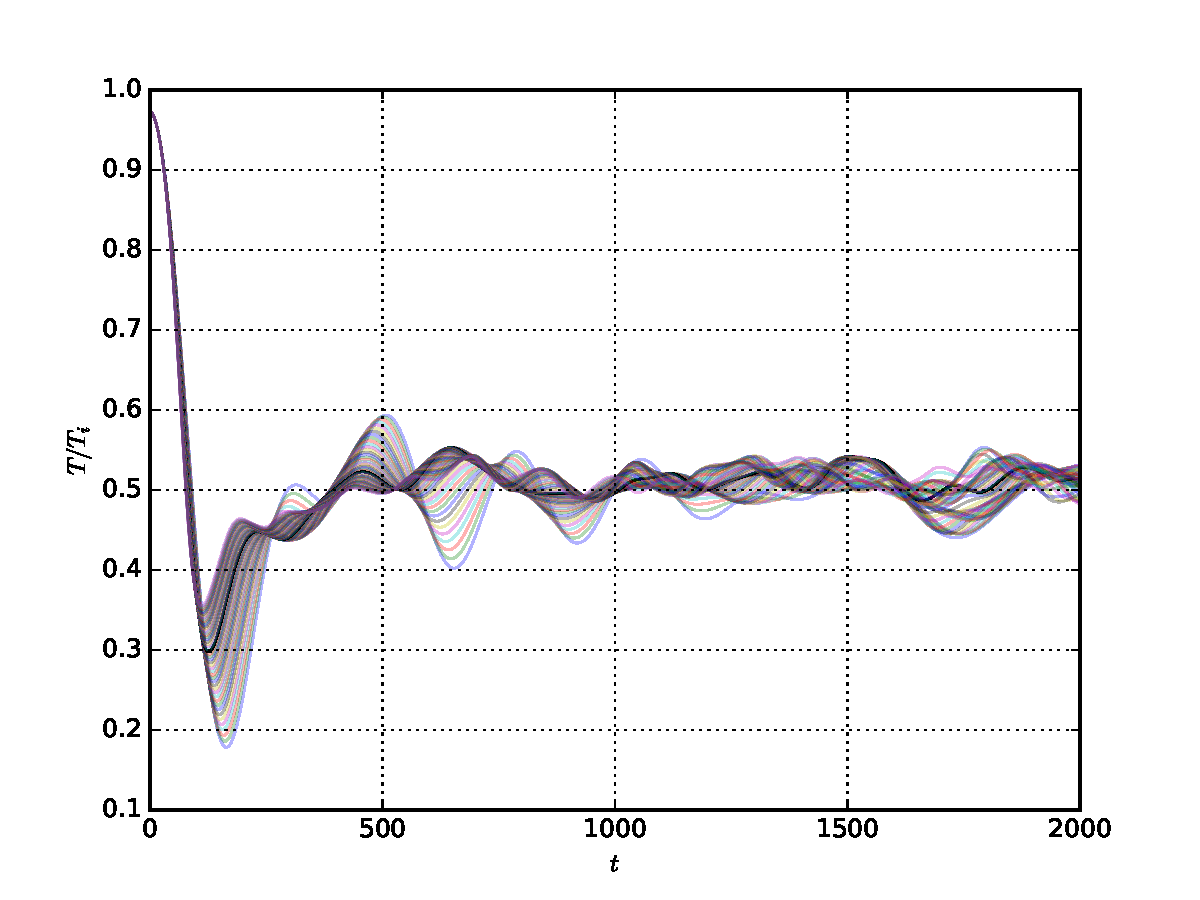
\includegraphics[width=\linewidth]{temperature_ratio.pdf}
    \caption[Temperature ratio]{Plotting the ratio between initial and
        instantaneous temperature for varying $T_i$. Here the initial
        temperatures ranges from 20 to 500 kelvin, with 48 intermediate steps.
    As we can see the ratio stabilizes around 0.5. The graph of an arbitrary
temperature has been highlighted in black.}
    \label{fig:temperature_ratio}
\end{figure}

\subsection{Melting temperature of system}
\label{sub:melting_temperature_of_system}

In order to measure the melting temperature of the system, we can use the Einstein relation which states the following:
\begin{equation}
    \notag
    \langle r^2(t) \rangle = 6Dt.
\end{equation}
$D$ is here the diffusion constant, $t$ is time and the \emph{mean square displacement} is calculated as
\begin{equation}
    \notag
    r_i^2(t) = \left| \vec{r}_i(t) - \vec{r}_i(0) \right|^2
\end{equation}
for atom $i$.

\clearpage

\begin{thebibliography}{9}
\bibitem{min_image}
    \url{https://en.wikipedia.org/wiki/Periodic_boundary_conditions#Practical_implementation:_continuity_and_the_minimum_image_convention}
\bibitem{equipar}
    \url{https://en.wikipedia.org/wiki/Equipartition\_theorem}
\bibitem{virial}
    \url{https://en.wikipedia.org/wiki/Virial_theorem}
\end{thebibliography}
\end{document}
